\documentclass[a4paper,10pt]{article}

\usepackage[utf8]{inputenc}
\usepackage{t1enc}

\usepackage[utf8]{inputenc}
\usepackage{t1enc}
\usepackage[spanish]{babel}
\usepackage[pdftex,usenames,dvipsnames]{color}
\usepackage[pdftex]{graphicx}
\usepackage{enumerate}
\usepackage{amsmath}
\usepackage{amsfonts}
\usepackage{amssymb}
\usepackage[table]{xcolor}
\usepackage[small,bf]{caption}
\usepackage{float}
\usepackage{subfig}
\usepackage{listings}
\usepackage{bm}
\usepackage{times}

\begin{document}
\setcounter{secnumdepth}{5}
\setcounter{tocdepth}{5}

\renewcommand{\lstlistingname}{C\'odigo Fuente}
\lstloadlanguages{Octave}
\lstdefinelanguage{MyOctave}[]{Octave}{
        deletekeywords={beta,det},
        morekeywords={repmat}
}
\lstset{
        language=MyOctave,
        stringstyle=\ttfamily,
        showstringspaces = false,
        basicstyle=\footnotesize\ttfamily,
        commentstyle=\color{gray},
        keywordstyle=\bfseries,
        numbers=left,
        numberstyle=\ttfamily\footnotesize,
        stepnumber=1,
        framexleftmargin=0.20cm,
        numbersep=0.37cm,
        backgroundcolor=\color{white},
        showspaces=false,
        showtabs=false,
        frame=l,
        tabsize=4,
        captionpos=b,
        breaklines=true,
        breakatwhitespace=false,
        mathescape=true
}

%%%%%%%%%%%%%%%%%%%%%%%%%%%%%%%%%%
%%%%%%%% begin TITLE PAGE %%%%%%%%
%%%%%%%%%%%%%%%%%%%%%%%%%%%%%%%%%%
\begin{titlepage}
        \vfill
        \thispagestyle{empty}
        \begin{center}
                
\includegraphics{./images/itba_logo.png}
                \vfill
                \Huge{Big Data}\\
                \vspace{1cm}
                \Huge{Trabajo Pr\'actico 2}\\
        \end{center}
        \vfill
        \large{
        \begin{tabular}{lcr}
                Crespo, Alvaro && 50758 \\
                Petit, Alejandro && 48308\\
                Susnisky, Dario && 50592 \\
                Videla, Máximo && 51071\\
        \end{tabular}
}
        \vspace{2cm}
        \begin{center}
                \large{18 de noviembre de 2013}\\
        \end{center}
\end{titlepage}
\newpage

\setcounter{page}{1}

% \tableofcontents
% \newpage

\section{Presentación del problema}
El objetivo de este trabajo práctivo es el de implementar un proyecto que realice un procesamiento en tiempo real de datos obtenidos de \textit{Twitter}.
Los \textit{tweets} se van descargando mediante un cliente y son procesados a medida que llegan. Para esto se utiliza \textit{Flume} detectando cuando llegan nuevos \textit{tweets}.
Una vez encolados los \textit{tweets} por \textit{Flume}, \textit{Storm} es el encargado de procesarlos, implementando las métricas deseadas. Para este último punto, \textit{Storm}
toma ciertos datos de \textit{HBase} y finalmente vuelca los resultados de las métricas en una tabla en \textit{MySQL}.

A continuación se presenta un esquema general de la aplicación:

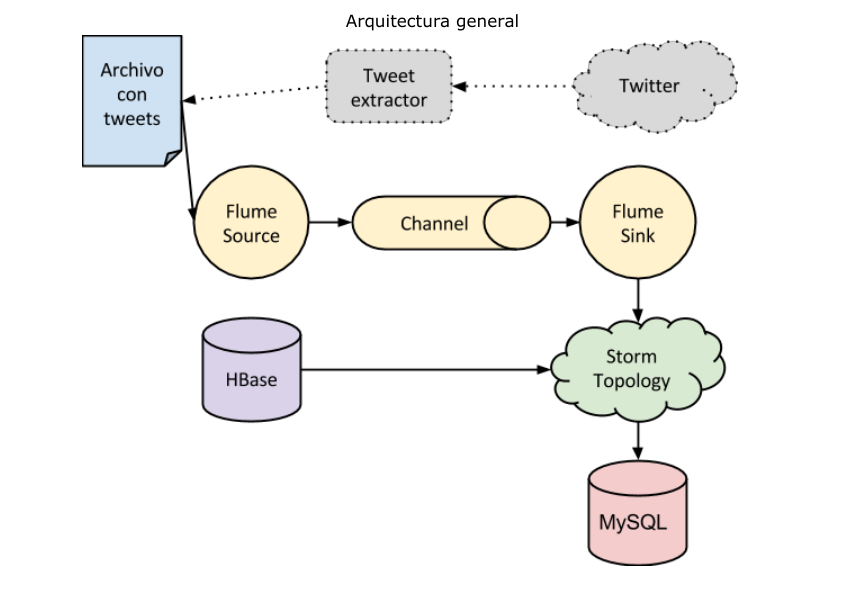
\includegraphics[width=\linewidth]{images/tp2BD.png}

\section{Decisiones de implementación}

\subsection{Agente de Flume}
Con respecto al agente de Flume se implementó un simple agente con un \textit{source}, 3 \textit{sinks} y 3 \textit{channels}, uno que vincule cada \textit{sink} con el
\textit{source}.

Para el \textit{source} se utilizó un \textit{Spooling Directory Source}, que viene dado en el paquete de Flume, que simplemente se queda observando un
determinado directorio y cuando se agregan nuevos archivos, genera un evento nuevo por cada línea. En nuestro caso, cada línea es un objeto JSON con la información de un tweet.

La decisión de tener varios \textit{sinks} vino por diferentes razones. En primer lugar, se utilizaron el \textit{Logger Sink} y el \textit{File Roll Sink}, que dirigen el output
del agente de Flume a consola (mediante logs de debugging de \textit{Log4j}) y a archivos de texto en un directorio de salida, respectivamente. Esto tenía el objetivo principal de
familiarizarnos con la nueva tecnología y a la vez ver el funcionamiento del \text{Spooling Directory Source} para nuestras necesidades. Pero luego también decidimos continuar
utilizandolas para testear y verificar el correcto funcionamiento del \textit{ActiveMQ Sink} que implementamos.

\subsection{Topología de Storm}

Al implementar una topología en Storm que permita medir nuestra métrica desarrollamos el siguiente modelo:
\begin{itemize}
  \item Un \textit{Spout} encargado de tomar los datos de la cola de mensajes.
  \item Un \textit{Bolt} que recibe todos los mensajes que envía el \textit{Spout} sin importar el orden.
		A su vez este \textit{Bolt} toma de \textit{HBase} todos los grupos de \textit{keywords} existentes y emite mensajes
		indicando cuántas menciones por grupo recibe por \textit{tweet}.
  \item Un último \textit{Bolt} que se encarga de sumar todos los mensajes que recibe y guardar la cantidad de menciones de cada grupo en una base de datos \textit{MySQL}.
\end{itemize}

El \textit{Spout} está unido al primer \textit{Bolt} mediante \textit{ShuffleGrouping} ya que no importa el orden de los mismos.
El primer \textit{Bolt} se encuentra unido al segundo con \textit{FilterGrouping} agrupando por el \textit{GroupId} ya que solamente un
\textit{Bolt} debe ser encargado de actualizar un element (en el ejemplo, uno de los partidos políticos) en la base de datos.

Para probar la topología se implementaron \textit{Bolts} que hacen sus tareas omitiendo las conexiones a \textit{MySQL} y \textit{HBase}.
Habiendo corroborado su correcto funcionamiento se implementaron luego, las versiones finales y completas.

\subsection{Cliente de Twitter}

\textit{Twitter} cuenta con 2 \textit{APIs} para consultar información. La primera es \textit{REST}, dandole a un desarrollador métodos para realizar pedidos HTTP apropiados,
que contengan como respuesta lo que se esta buscando. Por otro lado, \textit{Twitter} cuenta con una \textit{API} de \textit{streams} que encola \textit{tweets} (u otros eventos)
constantemente y con bajo costo, evitando el \textit{overhead} de la \textit{REST API}.

Dada la naturaleza y los requerimientos de la aplicación, fue casi intuitiva la decisión de utilizar la segunda \textit{API}. Contando con esto y con la decisión de desarrollar
la aplicación en \textit{Java}, se dicidió utilizar el cliente \textit{Hosebird} dado que proveía los servicios que buscabamos para nuestra aplicación (acceso a la
\textit{Streaming API}, autenticación vía \textit{Oauth} y otros). Además, \textit{Hosebird} permite integración sencilla con \textit{Maven} y nos dió la serguridad de tener
una prueba funcional en poco tiempo.

\section{Problemas encontrados}

\subsection{Agente de Flume}
El principal problema, o desafío, de la implementación del agente de Flume fue la necesidad de implementar un \textit{Sink} custom, para interactuar con la cola
de \textit{AciveMQ}, ya el tanto para el \textit{Souce} como para los \textit{Channels}, utilizamos implementaciones como \text{Spooling Directory Source} o \textit{Memory Channel},
que ya vienen provistas por Flume.

Un problema, o una lección, que tuvimos con Flume fue que si bien es posible que un \textit{source} se conecte a varios \textit{channels}, no sucede lo mismo con los \textit{sinks}.
Un \textit{sink} puede estar conectado a un y sólo un \textit{channel}. Además, al configurar el \textit{source} de nuestro agente con varios \textit{channels}, lo que
se denomina \textit{Fan Out Flow}, nos topamos con las
diferentes formas en que un source puede estar configurado para manejar conexiones a varios \textit{channels}, o la ``política de Fan Out''. Existen dos formas o políticas para esto:
replicar o multiplexar. En el primer caso, el \textit{source} le manda el evento generado a todos los \textit{channels} conectados, mientrás que en el segundo, el evento se envía
a un subconjunto de ellos. En nuestro caso, nos topamos con un error al configurar varios \textit{channels} ya que, al parecer, el default en estos casos es multiplexar, lo cual no
era lo que necesitabamos.

\subsection{Topología de Storm}

La configuración de \textit{Storm} para encontrar \textit{activeMQ} en modo distribuido nos presentó un desafío importante. Si bien contabamos con la configuración local,
al comenzar a probar la aplicación en modo distribuido nos encontramos diversas complicaciones.

Por otra parte, al implementar la topología, no fueron triviales las conexiones entre \textit{Spouts} y \textit{Bolts} ya que dependiendo del caso, requerían agrupaciones
diferentes. Finalmente logramos encontrar agrupaciones que permitiesen llegar a nuestro objetivo.

\subsection{Cliente de Twitter}

Si bien en la versión final del proyecto se utilizó \textit{Hosebird client}, en un comienzo se intentó utilizar la librería \textit{Twitter4J}. En un principio, esta librería,
parecía una potente posibilidad para consultar la \textit{Twitter API}. Finalmente se decidió utilizar \textit{Hosebird client} ya que provee una mejor documentación y un enfoque
completo en la \textit{Streaming API} en vez de la \textit{REST API} (que es la que finalmente se decidió usar).

\section{Instrucciones para ejecutar la métrica}

El proyecto cuenta con 3 partes que deben ejecutarse de manera paralela.
Se considera para la compilación de las 3 partes, que \textit{Maven} se encuentra instalado en el sistema.

\subsection{Cliente de Twitter}

\subsubsection{Compilación}

Para compilar el proyecto del consumidor de streams de \textit{Twitter} correr dentro de la carpeta tweetsStream:
\\

    mvn clean package
\\
\\
Para que el proyecto se compile de forma correcta, en la carpeta /tweetsStream/src/main/resources debe existir el archivo oauthcredentials con el siguiente formato:
\\

consumerKey = xxxxxxxx

consumerSecret = xxxxxxx

accessToken = xxxxxxx

accessTokenSecret = xxxxxxxx

\subsubsection{Ejecución}

Para correr el consumidor de streams de \textit{Twitter} correr dentro de la carpeta tweetsStream/target:
\\

	java -jar bigdata-twitterclient-jar-with-dependencies.jar <outputFolder> <terms>
\\
\\
El parámetro <outputFolder> es el path relativo de la carpeta en donde se crearan los archivos de salida. Esta carpeta debe existir previamente.
Paralelamente <terms> es la lista de términos a buscar separados por comas (","). Un ejemplo de términos podría ser "termino1,termino2,termino de prueba".

\subsection{Flume}

Se requiere que \textit{Flume} se encuentre instalado y agregado a la variable de entorno PATH.
Esto último se puede hacer de la siguiente manera:
\\

export PATH=absolute-path/to/flumeDir/bin:\$PATH
\\
\\
Para verificar que \textit{Flume} está agregado al PATH se debería poder correr desde la consola el comando ``flume-ng`` y
verificar que el output es el del comando en cuestión.

\subsubsection{Compilación}

Para compilar el proyecto \textit{Flume} con el custom sink para activeMQ correr dentro de la carpeta flume
\\

	mvn clean package -DskipTests

\subsubsection{Ejecución}

Para correr el agente de \textit{Flume} correr dentro de la carpeta flume
\\

	sh run-flume.sh
\\
\\
La configuración del agente de \textit{Flume} se encuentra en la carpeta flume/conf.

\subsection{Storm}

\subsubsection{Compilación}

Para compilar el proyecto \textit{Storm} con la topología correr dentro de la carpeta storm
\\

	mvn clean package

\subsubsection{Ejecución}

Para correr la topología de \textit{Storm} correr dentro de la carpeta storm
\\

	storm jar target/storm-0.0.1-SNAPSHOT-jar-with-dependencies.jar com.itba.g2.storm.StormTopology topologyName sqlDBUrl table mainField countField user pass columnFamily
\\
\\
Los parámetros son los siguientes:

\begin{itemize}
	\item ``topologyName`` es el nombre que se le quiere dar a la topología de storm que se correrá.
	\item ``sqlDBUrl`` es la url de la base de datos \textit{MySQL} donde se escribirán los resultados.
	\item ``table`` es el nombre de la tabla donde se almacenarán los resultados.
	\item ``mainField`` es el campo de la tabla que representa el nombre de la agrupación.
	\item ``countField`` es el campo de la tabla que representa la cantidad de menciones.
	\item ``user`` es el usuario para acceder a la base de datos \textit{MySQL}.
	\item ``pass`` es la usuario para acceder a la base de datos \textit{MySQL}.
	\item ``columnFamily`` es el nombre de la columna de la tabla de \textit{HBase} que contiene las palabras a buscar.
\end{itemize}

Una vez ejecutada una topología, si se desea volverla a correrla (con el mismo nombre) se debe dar de baja previamente la topología anterior. Esto se logra corriendo
\\

	storm kill topologyName

\subsection{Consideraciones}

\subsubsection{ActiveMQ}

Tanto el proyecto \textit{Flume} como el de \textit{Storm} utilizan una cola de mensaje \textit{ActiveMQ}, que debe estar correctamente instalado,
y cuya url es uno de los parámetros para correr el proyecto de \textit{Storm}.

Para monitorear el funcionamiento de las colas en ActiveMQ se puede acceder a
[http://hadoop-2013-datanode-2:8161/admin/queues.jsp](http://hadoop-2013-datanode-2:8161/admin/queues.jsp)

\small
\section{Formato de los resultado de la métrica}

Los resultados de la métrica implementada se almacenan en una tabla de MYSQL, conforme a los requerimientos de la cátedra. El esquema que definimos para esta tabla consiste
simplemente de los campos:

\begin{itemize}
    \item GroupId: El nombre del grupo o conjunto de palabras de interés
    \item Ammount: La cantidad de menciones de palabras relacionadas con el grupo
\end{itemize}


\end{document}
